\documentclass[article]{jss}

%% -- LaTeX packages and custom commands ---------------------------------------

%% recommended packages
\usepackage{thumbpdf,lmodern}

%% additional packages
\usepackage{amssymb,amsmath}

%% new custom commands
\newcommand{\class}[1]{`\code{#1}'}
\newcommand{\fct}[1]{\code{#1()}}

%% For Sweave-based articles about R packages:
%% need no \usepackage{Sweave}



%% -- Article metainformation (author, title, ...) -----------------------------

%% - \author{} with primary affiliation
%% - \Plainauthor{} without affiliations
%% - Separate authors by \And or \AND (in \author) or by comma (in \Plainauthor).
%% - \AND starts a new line, \And does not.
\author{Lennart Oelschl\"ager \\Bielefeld University \And Timo Adam \\University of St Andrews\And Rouven Michels \\Bielefeld University}
\Plainauthor{Lennart Oelschl\"ager, Timo Adam, Rouven Michels}

%% - \title{} in title case
%% - \Plaintitle{} without LaTeX markup (if any)
%% - \Shorttitle{} with LaTeX markup (if any), used as running title
\title{\pkg{fHMM}: Hidden Markov Models for Financial Time Series in \proglang{R}}
\Plaintitle{fHMM: Hidden Markov Models for Financial Time Series in R}
\Shorttitle{fHMM}

\Abstract{
%% Intro to HMMs
Hidden Markov models constitute a versatile class of statistical models for time series that are driven by hidden states. In financial applications, the hidden states can often be linked to market regimes such as bearish and bullish markets or recessions and periods of economics growth. To give an example, when the market is in a nervous state, corresponding stock returns often follow some distribution with relatively high variance, whereas calm periods are often characterized by another distribution with relatively smaller variance. Hidden Markov models can be used to explicitly model the distributions of the observations conditional on the hidden states and the transitions between states, and thus help us to draw a comprehensive picture of market behavior.
%% Intro to the package
In this paper, we introduce the \proglang{R} package \pkg{fHMM}, which provides various tools for applying hidden Markov models to financial time series. It provides functions for fitting hidden Markov models to empirical data, conducting simulation experiments, and decoding the underlying state sequence. Furthermore, functions for model checking, model selection, and state prediction are provided. In addition to basic hidden Markov models, hierarchical hidden Markov models are implemented. Its aim is to give \proglang{R} users interested in financial applications access to hidden Markov models and their extensions.
}

%% - \Keywords{} with LaTeX markup, at least one required
%% - \Plainkeywords{} without LaTeX markup (if necessary)
%% - Should be comma-separated and in sentence case.
\Keywords{hidden Markov models, regime switching, financial time series, decoding market behavior, \proglang{R}}
\Plainkeywords{hidden Markov models, regime switching, financial time series, decoding market behavior, R}

%% - \Address{} of at least one author
%% - May contain multiple affiliations for each author
%%   (in extra lines, separated by \emph{and}\\).
%% - May contain multiple authors for the same affiliation
%%   (in the same first line, separated by comma).
\Address{
  Lennart Oelschl\"ager\\
  Department of Business Administration and Economics\\
  Bielefeld University\\
  Postfach 10 01 31, Germany\\
  E-mail: \email{lennart.oelschlaeger@uni-bielefeld.de}\\ \\
  Timo Adam \\
  School of Mathematics and Statistics\\
  University of St Andrews\\
  The Observatory, Buchanan Gardens, St Andrews KY16 9LZ, UK\\
  E-mail: \email{ta59@st-andrews.ac.uk}\\ \\
  Rouven Michels \\
  Department of Business Administration and Economics\\
  Bielefeld University\\
  Postfach 10 01 31, Germany\\
  E-mail: \email{r.michels@uni-bielefeld.de}
}

\begin{document}
%% Do we need to following line?
%% \SweaveOpts{concordance=TRUE}

%% -- Introduction -------------------------------------------------------------

%% - In principle "as usual".
%% - But should typically have some discussion of both _software_ and _methods_.
%% - Use \proglang{}, \pkg{}, \fct{} and \code{} markup throughout the manuscript.
%% - If such markup is in (sub)section titles, a plain text version has to be
%%   added as well.
%% - All software mentioned should be properly \cite-d.
%% - All abbreviations should be introduced.
%% - Unless the expansions of abbreviations are proper names (like "Journal
%%   of Statistical Software" above) they should be in sentence case (like
%%   "generalized linear models" below).

\section{Introduction}
\label{sec:intro} %% Timo 

%% Intro to HMMs
In recent years, Hidden Markov models (HMMs) have emerged as a popular tool for modeling time series that are subject to state-switching over time \citep{zuc16}. In their basic form, HMMs comprise an observed state-dependent process that is driven by a hidden state process, the latter of which is typically modeled using a discrete-time, finite-state Markov chain. In financial applications, the states of the underlying Markov chain can often be linked to market regimes such as bearish and bullish markets or recessions and periods of economics growths. To give an example, when the market is in a nervous state, corresponding stock returns often follow some distribution with relatively high variance, whereas when the market is in a clam state, another distribution with relatively smaller variance is active. By their dependence structure, HMMs naturally account for such disparate patterns and thus allow us to infer hidden market regimes and their underlying dynamics from financial time series.

%% Literature review
Over the last decades, HMMs have become increasingly popular in finance. In various studies, they have been applied to model business cycles \citep{kim98, gre00}, to derive stylized facts of stock returns \citep{bul06, nys15a}, and to model energy prices conditional on market regimes \citep{lan18, ada19c, ada22}, to name but a few examples. \cite{lih17} used HMMs to model volatility in the Standard and Poor's 500 index to investigate the conjecture that stock returns exhibit negative correlation with volatility. \cite{ngu18} used HMMs to predict closing prices to derive an optimal trading strategy, which was shown to outperform the conventional buy-and-hold strategy, whereas \cite{bul11, nys15a, nys18} have shown that HMMs prove useful in asset allocation and portfolio optimization applications. All these examples demonstrate that HMMs constitute a versatile class of statistical models for time series that naturally accounts for the state-switching patterns often found in financial data.

%% Software overview
In \proglang{R} \citep{r21}, various implementations of HMMs are available. For general purposes, the packages \pkg{hmm} \citep{him10}, \pkg{depmixS4} \citep{vis10}, and \pkg{msm} \citep{jac11} are frequently used. In addition, a wide range of special-purpose packages is available, for example \pkg{moveHMM} \citep{mic16} and \pkg{momentuHMM} \citep{mcc18} for modeling ecological time series, \pkg{hsmm} \citep{bul10} and \pkg{mhsmm} \citep{oco11} for hidden semi-Markov models, \pkg{hmm.discnp} \citep{tur14} and \pkg{countHMM} \citep{ada19b} for modeling count data, and \pkg{LMest} \citep{bar17} for modeling longitudinal data. In \proglang{Python}, the library \pkg{hmmlearn} \citep{leb22} can be used. Yet, an \proglang{R} package tailored to financial applications is still lacking.

%% Intro to the package
In this paper, we introduce the \proglang{R} package \pkg{fHMM} \citep{oel22}, which aims to complement the above mentioned collection by making HMMs accessible to \proglang{R} users with a special interest in financial time series. The package functionality can be classified into functions for data preparation, model estimation, and model evaluation, which are illustrated in the flowchart displayed in Figure \ref{fig:flowchart}. 
\begin{figure}[t!]
  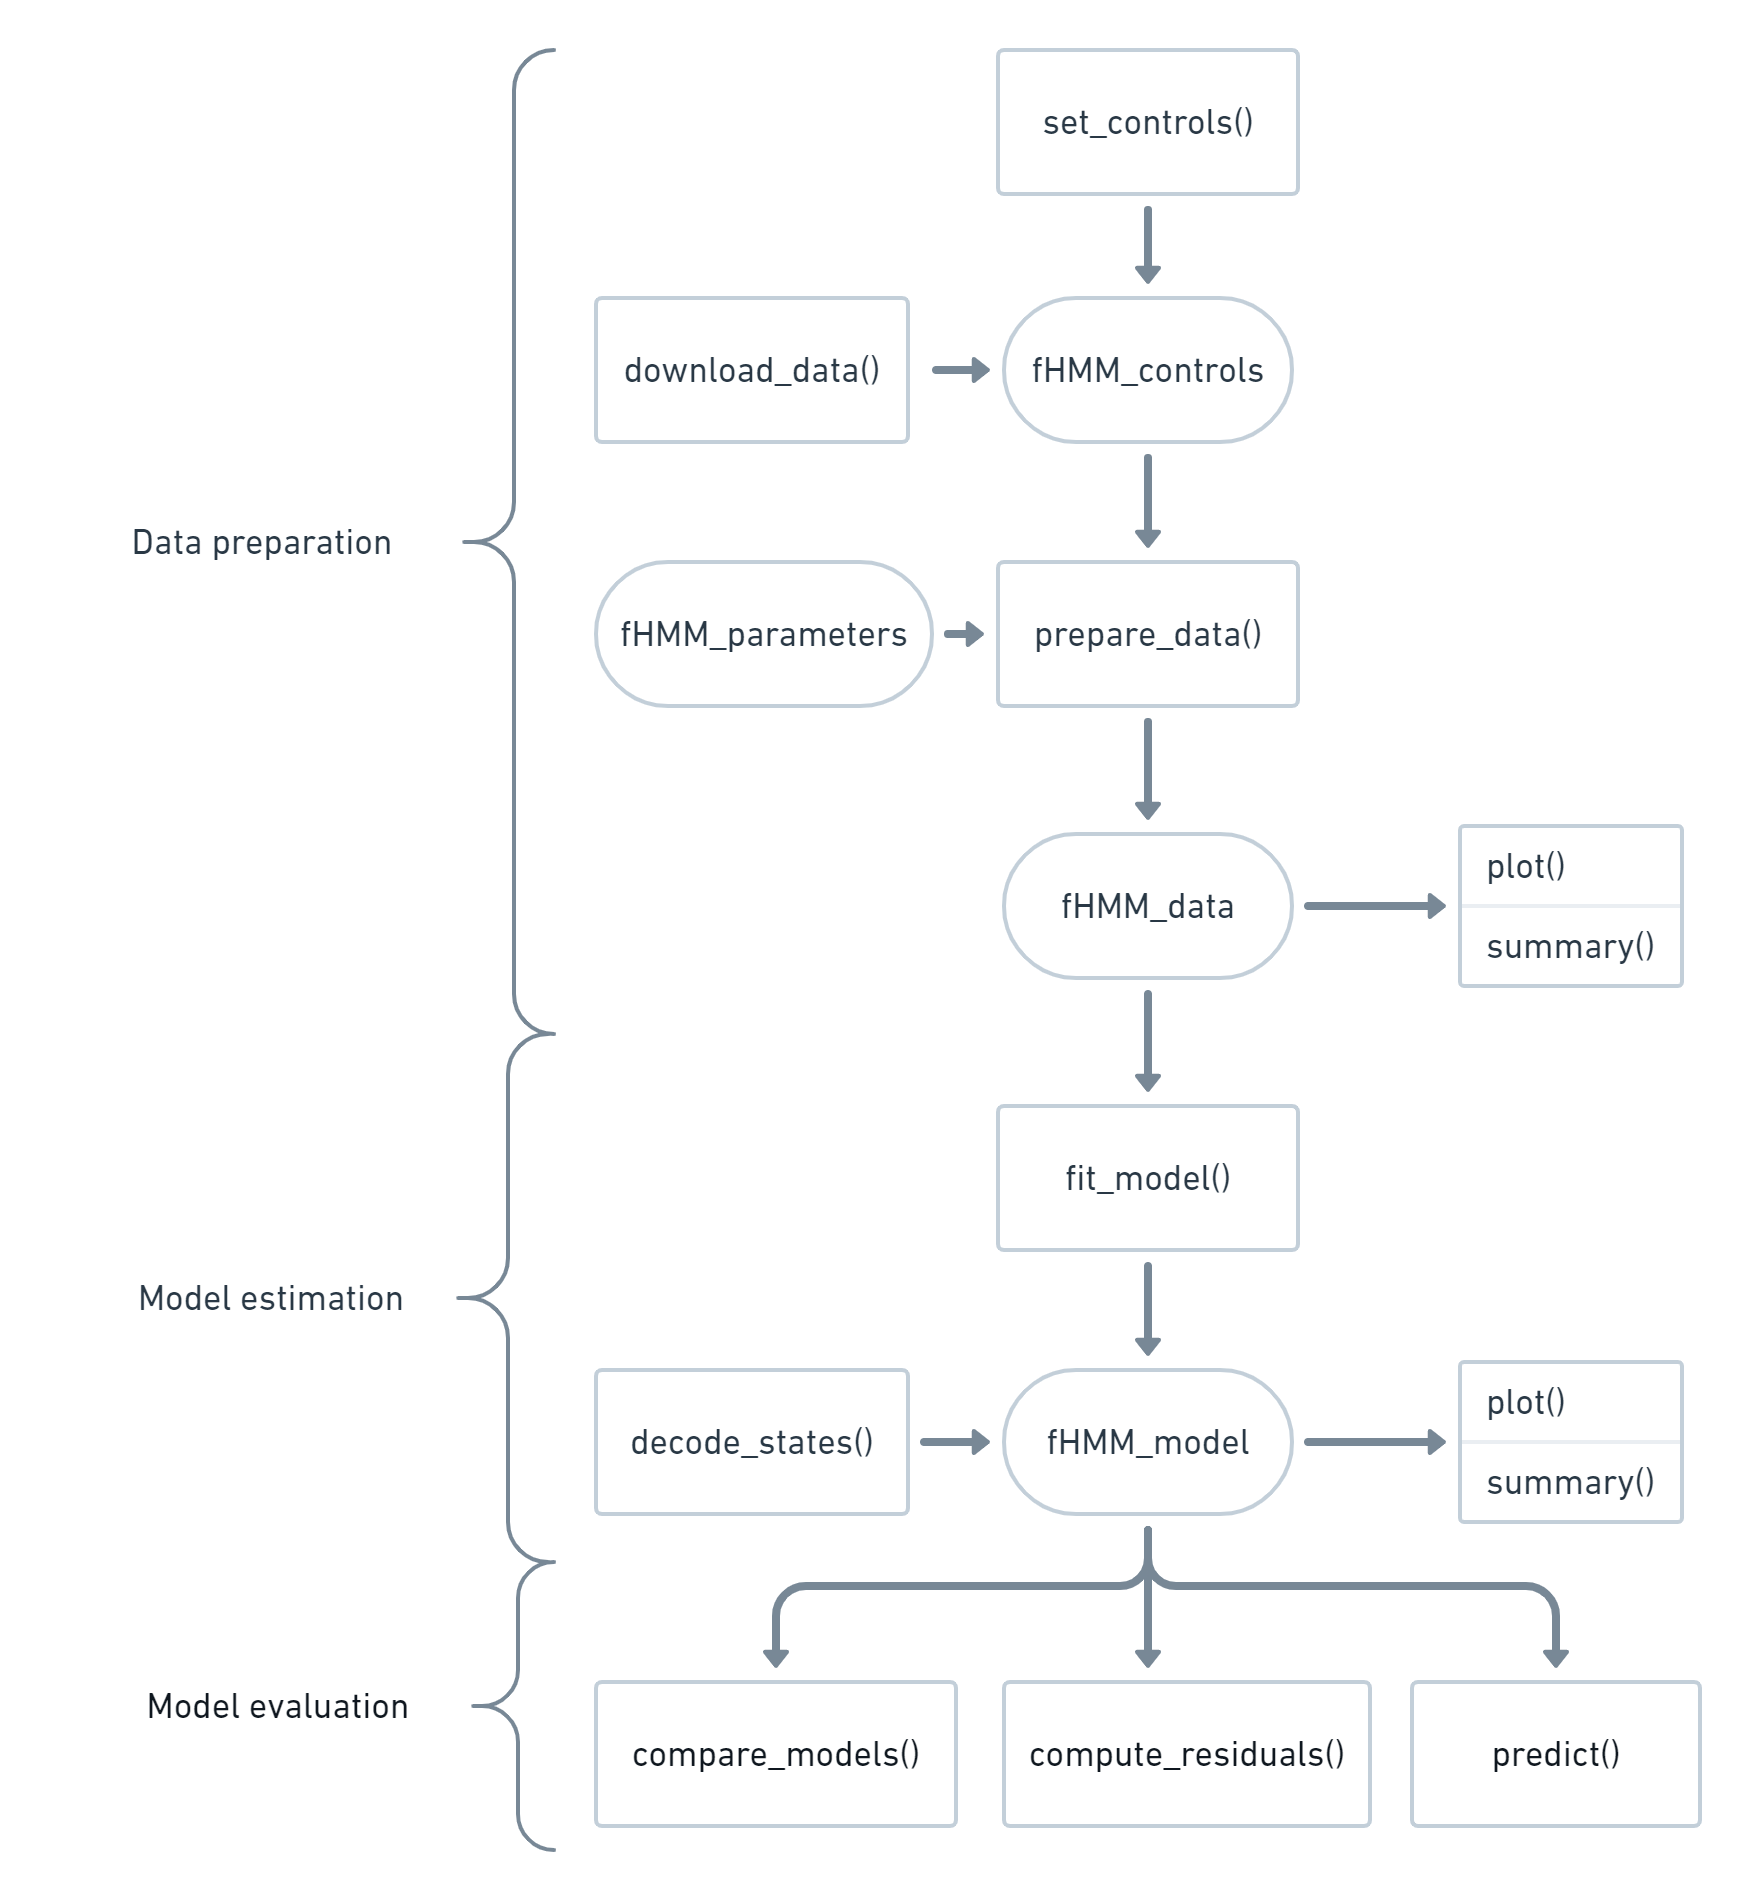
\includegraphics{flowchart.png}
  \caption{Package flowchart. The main functions are visualized using rectangles, while objects are illustrated as ovals.}
  \label{fig:flowchart}
\end{figure}
Functions for data preparation include a convenient interface to Yahoo Finance (https://www.finance.yahoo.com) that allows users to download stock market data. The model is estimated in a maximum likelihood framework, where the likelihood is evaluated using the forward algorithm, which is implemented in \proglang{C++} and parallelized for fast and efficient computation. Functions for model evaluation include pseudo-residual analyses and the computation of model selection criteria. The package also implements hierarchical HMMs; an extension of basic HMMs proposed in \cite{oel21} that improves the model's capability of distinguishing between short- and long-term trends and allows us to jointly model data streams collected at different time scales, such as monthly trade volumes and daily stock returns \citep{ada20}. 

%% Outline of the paper
The paper is structured as follows: in Section 2, we introduce HMMs, focusing on their dependence structure and model assumptions. In Sections 3--8, we illustrate a typical workflow using the \pkg{fHMM} package, where we explain how to specify the model, how to download, prepare, and simulate data, how to fit the model, how to decode the hidden states, how to use a fitted model for state forecasting, how to check the goodness of fit, and how to perform model selection. Each section begins with some theoretical background, which is followed by illustrating examples using simulated data, stock index data from the Deutscher Aktienindex (DAX), and stock market data from the Volkswagen Group (VW). Each of these sections is complemented by code chunks, which cannot only be used to replicate the examples given but also serve as a starting point for users who want to apply HMMs to their own data. Section 9 concludes and gives an outlook of anticipated package extensions.

%% -- Manuscript ---------------------------------------------------------------

%% - In principle "as usual" again.
%% - When using equations (e.g., {equation}, {eqnarray}, {align}, etc.
%%   avoid empty lines before and after the equation (which would signal a new
%%   paragraph.
%% - When describing longer chunks of code that are _not_ meant for execution
%%   (e.g., a function synopsis or list of arguments), the environment {Code}
%%   is recommended. Alternatively, a plain {verbatim} can also be used.
%%   (For executed code see the next section.)
%% - Tables are placed at the top of the page
%%   (\verb|[t!]|), centered (\verb|\centering|), with a caption below the table,
%%   column headers and captions in sentence style, and if possible avoiding
%%   vertical lines.
%% - Virtually all JSS manuscripts list source code along with the generated
%%   output. The style files provide dedicated environments for this.
%% - In R, the environments {Sinput} and {Soutput} - as produced by Sweave() or
%%   or knitr using the render_sweave() hook - are used (without the need to
%%   load Sweave.sty).
%% - Equivalently, {CodeInput} and {CodeOutput} can be used.
%% - The code input should use "the usual" command prompt in the respective
%%   software system.
%% - For R code, the prompt "R> " should be used with "+  " as the
%%   continuation prompt.
%% - Comments within the code chunks should be avoided - these should be made
%%   within the regular LaTeX text.
%% - Please make sure that all code is properly spaced, e.g., using
%%   \code{y = a + b * x} and \emph{not} \code{y=a+b*x}.
%% - JSS prefers when the second line of code is indented by two spaces.

\section{Model definition} \label{sec:model_definition} %% Rouven

Hidden Markov models (HMMs) constitute a modeling framework for time series where a sequence of observations is assumed to depend on a hidden state process. The peculiarity is that, instead of the observation process, the state process cannot be directly observed. However, the hidden states comprise information about the environment the model is applied on. The hidden state process and the observed state-dependent process are connected as follows: we assume that for each point in time $t = 1, \ldots, T$, an underlying process $(S_t)_{t = 1, \ldots, T}$ is in one of $N$ possible states. Then, depending on the active state $S_t \in \{ 1, \ldots, N \}$, the observation $X_t$ from the state-dependent process $(X_t)_{t = 1, \ldots, T}$ is assumed to be generated by the corresponding state-dependent distribution $f^{(S_t)}$. We assume $(S_t)_t$ to be Markovian, i.e.\ the active state at time $t$ only depends on the previous state at time $t-1$. Henceforth, the state process is identified by its initial distribution $\delta = (\delta_i), \delta_i = \Pr(S_1 = i), i = 1, \ldots, N$, and its transition probability matrix (t.p.m.) $\Gamma = (\gamma_{i,j}), \gamma_{i,j} = \Pr(S_{t} = j|S_{t-1}=i), i,j = 1, \ldots, N, t = 2, \ldots, T$. Furthermore, $(X_t)_{t = 1, \ldots, T}$ satisfies the conditional independence assumption, i.e.\ the observation $X_t$ depends on the current state $S_t$, but is independent from previous observations or states.

When modeling financial time series, the different states can serve as proxies for the current market situation, e.g.\ calm and nervous. Even though these moods cannot be directly observed, price changes or trading volumes (which can be assumed to depend on the current mood of the market) are observable. Thereby, using an underlying Markov process, we can detect which mood is active at any point in time and how the different moods alternate. Depending on the current mood, a price change is generated by a different distribution. These distributions characterize the moods in terms of expected return and volatility. For example, we can explicitly model price changes at time $t$ by different normal distributions whose mean and variance depend on the current state, $S_t$.

Following \cite{zuc16}, we assume that the initial distribution $\delta$ equals the stationary distribution $\pi$, where $\pi = \pi \Gamma$, i.e.\ the stationary and henceforth the initial distribution is determined by $\Gamma$.\footnote{A note on the existence of a stationary distribution: If the Markov process is irreducible, it has a unique distribution, which is the solution to the equation system $\pi = \pi \Gamma$. If, additionally, the Markov process is aperiodic, its state distribution converges to the stationary distribution, see \cite{nor97}. Irreducibility and aperiodicity are usually satisfied in practice.} This is reasonable from a practical point of view: On the one hand, the hidden state process has been evolving for some time before we start to observe it and hence can be assumed to be stationary. On the other hand, setting $\delta=\pi$ reduces the number of parameters that need to be estimated, which is convenient from a computational perspective.

The hierarchical hidden Markov model (HHMM) is a flexible extension of the basic HMM that can jointly model data observed on two different time scales \citep{oel21}. The two time series, one on a coarser and one on a finer scale, differ in the number of observations, e.g.\ monthly observations on the coarser scale and daily observations on the finer scale. Following the concept of HMMs, we can model both state-dependent time series jointly. First, we treat the time series on the coarser scale as stemming from an ordinary HMM, which we refer to as the coarse-scale HMM: At each time point $t$ of the coarse-scale time space $\{1,\dots,T\}$, an underlying process $(S_t)_t$ selects one state from the coarse-scale state space $\{1,\dots,N\}$. We refer to $(S_t)_t$ as the hidden coarse-scale state process. Depending on which state is active at time $t$, one of $N$ possible distributions $f^{(1)},\dots,f^{(N)}$ realizes the observation $X_t$. The process $(X_t)_t$ is called the observed coarse-scale state-dependent process. The processes $(S_t)_t$ and $(X_t)_t$ have the same properties as before, namely $(S_t)_t$ is a first-order Markov process and $(X_t)_t$ satisfies the conditional independence assumption. This dependence structure is visualized in the upper part of Figure \ref{fig:hhmm}.

Subsequently, we segment the observations of the fine-scale time series into $T$ distinct chunks, each of which contains all data points that correspond to the $t$-th coarse-scale time point. Assuming that we have $T^*$ fine-scale observations on every coarse-scale time point, we face $T$ chunks, each comprising $T^*$ fine-scale observations. The hierarchical structure now evinces itself as we model each of the chunks by one of $N$ possible fine-scale HMMs. Each of the fine-scale HMMs has its own t.p.m.\ $\Gamma^{*(i)}$, initial distribution $\delta^{*(i)}$, stationary distribution $\pi^{*(i)}$, and state-dependent distributions $f^{*(i,1)},\dots,f^{*(i,N^*)}$. Which fine-scale HMM is selected to model the $t$-th chunk of fine-scale observations depends on the hidden coarse-scale state $S_t$. The $i$-th fine-scale HMM explaining the $t$-th chunk of fine-scale observations consists of the following two stochastic processes: At each time point $t^*$ of the fine-scale time space $\{1,\dots,T^*\}$, the process $(S^*_{t,t^*})_{t^*}$ selects one state from the fine-scale state space $\{1,\dots,N^*\}$. Depending on which state is active at $t^*$, one of $N^*$ possible distributions $f^{*(i,1)},\dots,f^{*(i,N^*)}$ realizes the observation $X^*_{t,t^*}$. 

The fine-scale processes satisfy the Markov property and the conditional independence assumption, respectively, as well. Furthermore, it is assumed that the fine-scale HMM explaining $(X^*_{t,t^*})_{t^*}$ only depends on $S_t$. Figure \ref{fig:hhmm} visualizes the hierarchical dependence structure.

\begin{figure}
  \centering
  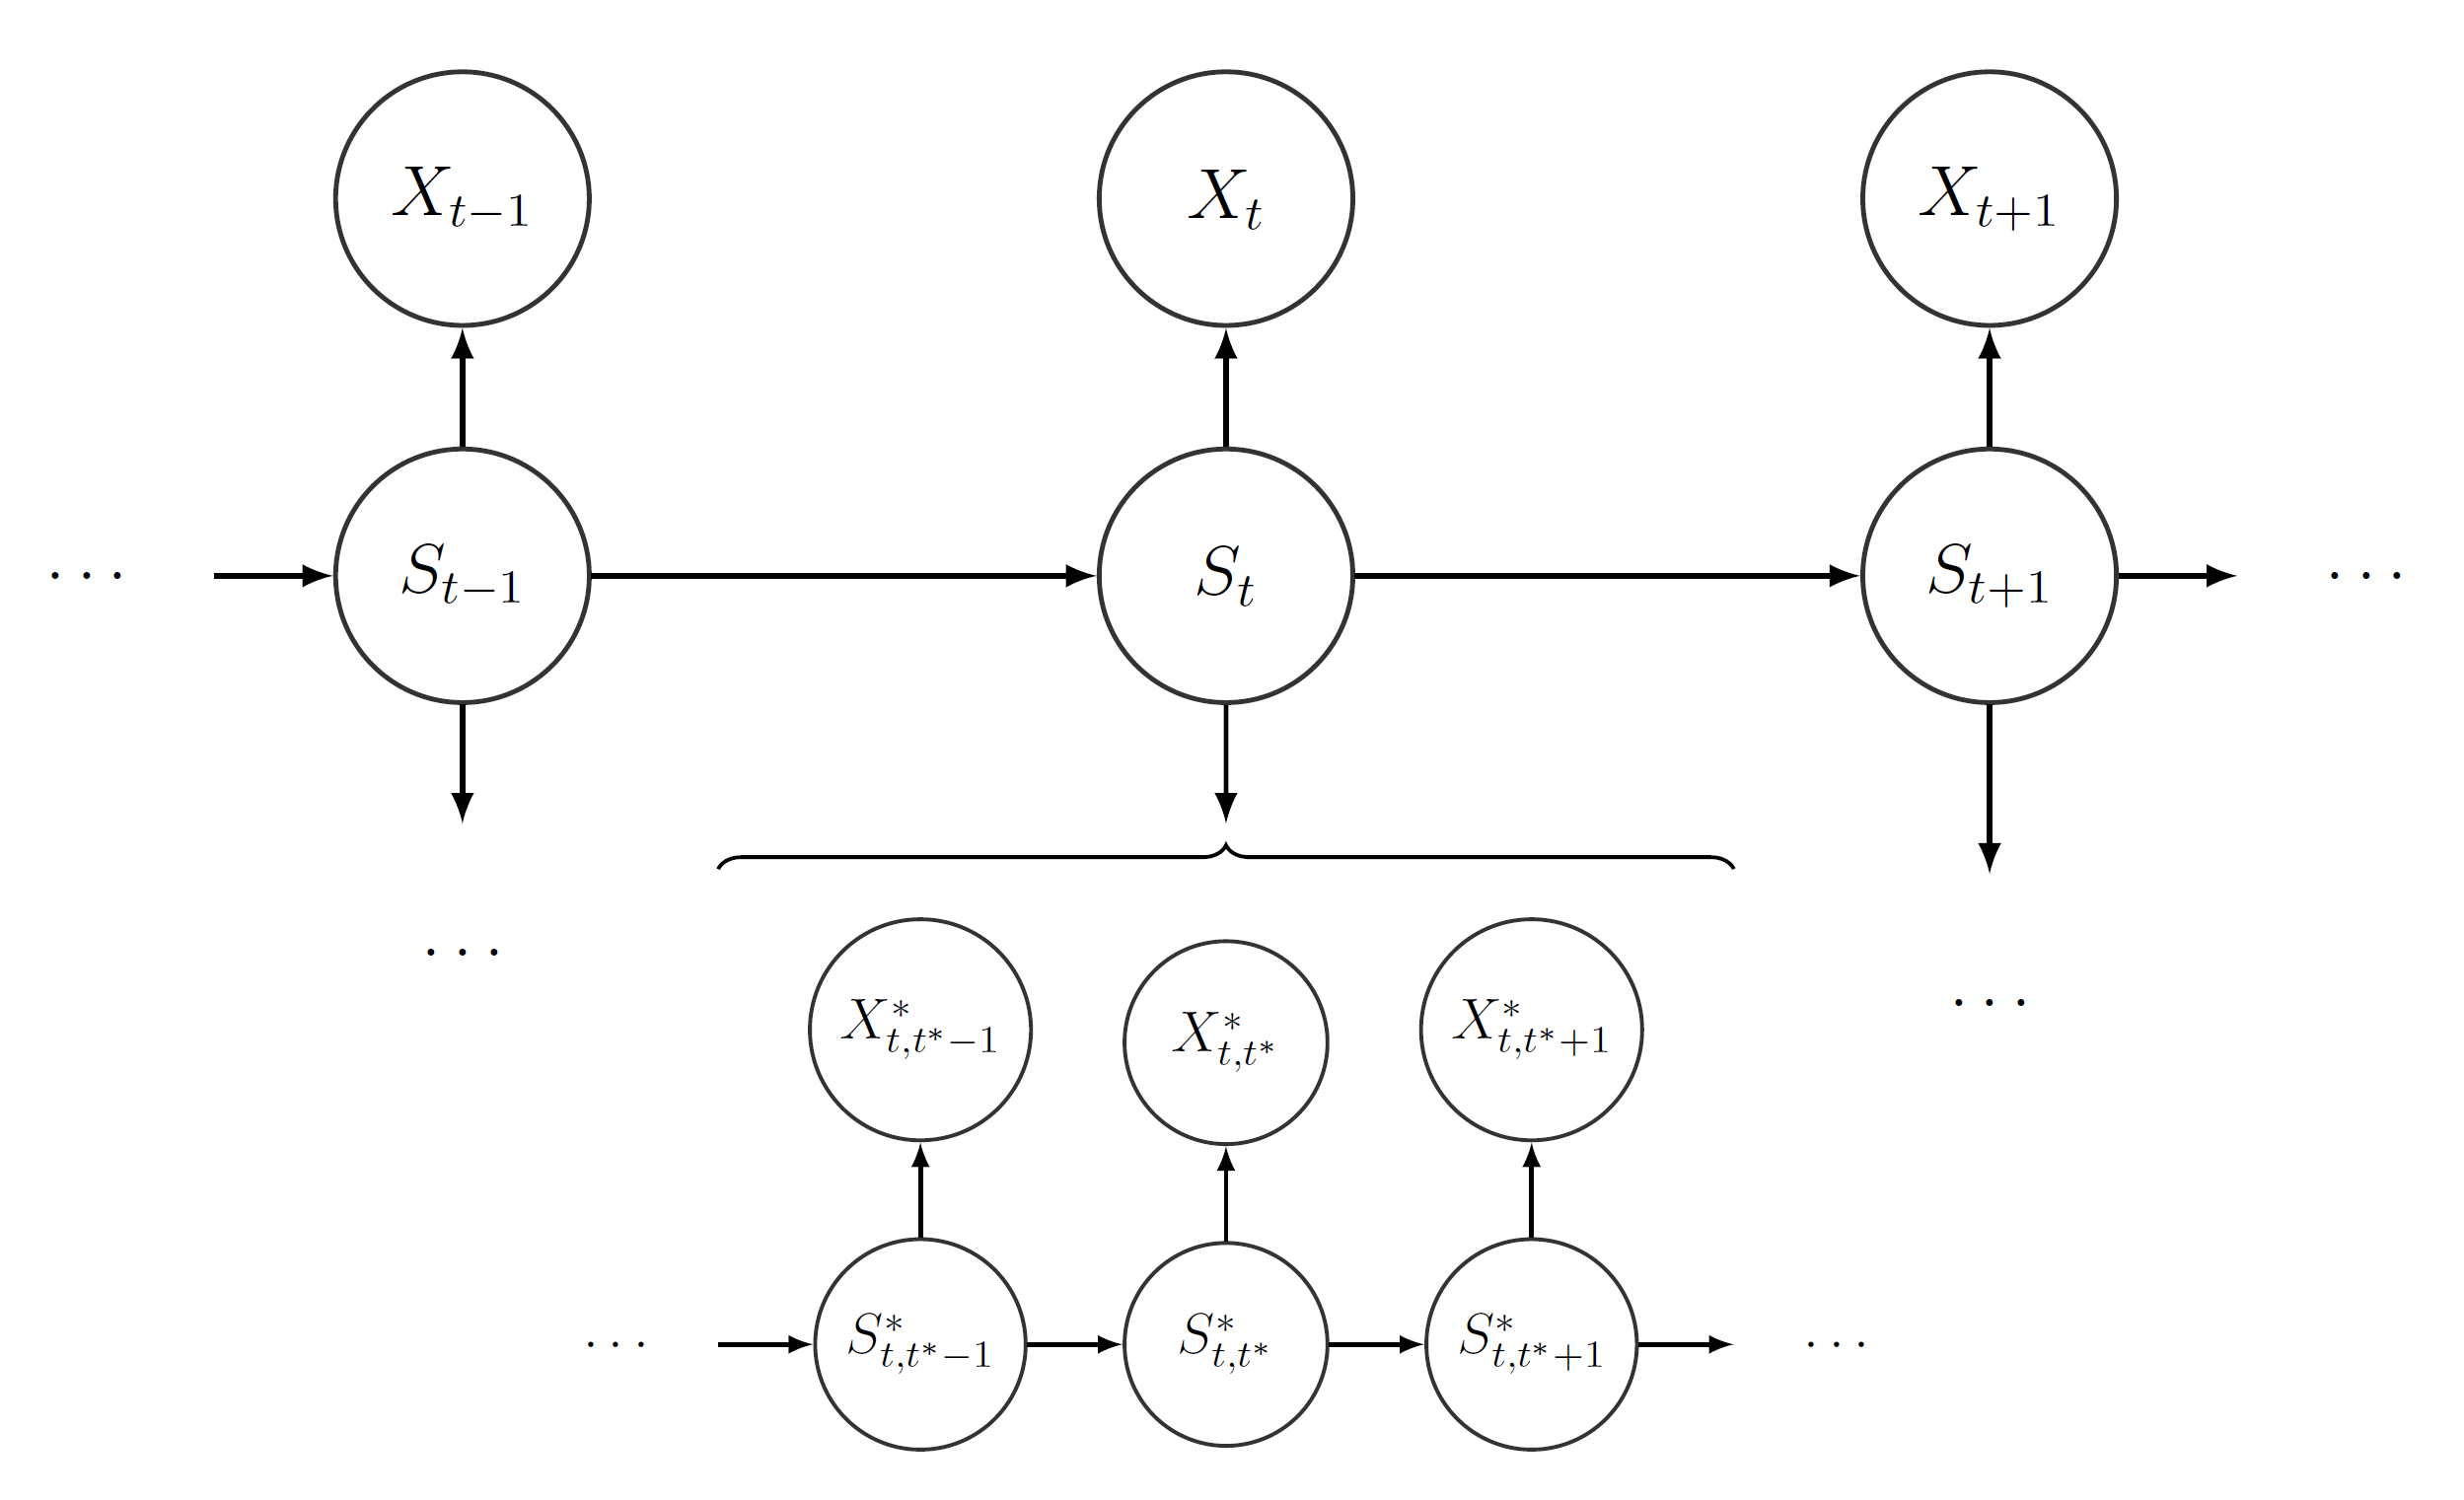
\includegraphics{hhmm.png}
  \caption{Dependence structure of an HHMM. The dependence structure of a basic HMM is visualized in the upper part.}
  \label{fig:hhmm}
\end{figure}

\section{Model specification} \label{sec:model_specification} %% Lennart

In the \pkg{fHMM} package, models are specified by a named list of controls that is passed to the \fct{set\_controls} function. This usually constitutes the first step when using the package, see Figure \ref{fig:flowchart}. The function checks the specifications and returns an \class{fHMM\_controls} object, which stores all settings and thereby provides the information required for other functionalities. In the following, we demonstrate three example specifications that should help the user to tailor an HMM to their need. The examples are continued in the following sections. All possible specifications are documented in detail on the function's help page, which can be accessed from the \proglang{R} console via \code{help(set_controls, package = "fHMM")}.

\paragraph{Example 1: DAX.} We fit a 3-state HMM to the closing prices of the DAX \citep{jan92}. Assume that the time series data is available in the working directory as file \code{"dax.csv"}. Such data can be obtained directly from Yahoo Finance via the convenience function \fct{download\_data}, see Section \ref{sec:data_management}.

The following lines set the number \code{states = 3} of hidden states. Any number greater than or equal to 2 is possible. Next, \code{sdds = "t"} specifies state-dependent t-distributions, which provides a popular choice for modeling log-returns \citep{pla08}. Alternatively, \code{sdds = "gamma"} specifies Gamma distributions, which is useful for model trading volumes as in \cite{ada20}. The \code{data} entry sets the path to the data file (\code{file = "dax.csv"}), the file's column that contains the dates (\code{date_column = "Date"}), and the data (\code{date_column = "Close"}). The specification \code{logreturns = TRUE} transforms the data to log-returns.

%
\begin{Schunk}
\begin{Sinput}
R> contr_dax <- list(
+    states = 3,
+    sdds   = "t",
+    data   = list(file        = "dax.csv",
+                  date_column = "Date",
+                  data_column = "Close",
+                  logreturns  = TRUE)
+  )
\end{Sinput}
\end{Schunk}
%

Passing this list to the \fct{set\_controls} function returns an object of class \class{fHMM\_controls}, which contains the specifications and default settings.

%
\begin{Schunk}
\begin{Sinput}
R> contr_dax <- set_controls(contr_dax)
R> class(contr_dax)
\end{Sinput}
\begin{Soutput}
[1] "fHMM_controls"
\end{Soutput}
\end{Schunk}
%

\paragraph{Example 2: Simulation.} If the \code{data} entry is not set, data will be simulated from the model specification. Simulation typically serves to assess the properties of estimation algorithms either for research or in a bootstrap like fashion, as seen for example in \cite{oel19}. The following lines specify a 2-state HMM with state-dependent Gamma distributions, where the expectation values for state 1 and 2 are fixed to \code{1} and \code{2}, respectively. The model will be fitted to 200 data points (\code{horizon = 200}) simulated from this specification based on \code{runs = 50} randomly initialized numerical optimization runs of the model's likelihood function. Printing the \class{fHMM\_controls} object summarizes the specification:

%
\begin{Schunk}
\begin{Sinput}
R> contr_sim <- list(
+    states  = 2,
+    sdds    = "gamma(mu = 1|2)",
+    horizon = 200,
+    fit     = list(runs = 50)
+  )
R> (contr_sim <- set_controls(contr_sim))
\end{Sinput}
\begin{Soutput}
fHMM controls:
* hierarchy: FALSE 
* data type: simulated 
* number of states: 2 
* sdds: gamma(mu = 1|2) 
* number of runs: 50  
\end{Soutput}
\end{Schunk}
%

\paragraph{Example 3: Hierarchy.} An HHMM can be specified by adding \code{hierarchy = TRUE} to the controls. The following is a specification for the DAX on the fine scale and the VW stock on the coarse scale (both data sets are contained in \pkg{fHMM}): 

%
\begin{Schunk}
\begin{Sinput}
R> contr_hhmm <- list(
+    hierarchy = TRUE,
+    states    = c(2,2),
+    sdds      = c("t(df = 1)", "t(df = 1)"),
+    period    = "m",
+    data      = list(file = c(system.file("extdata", "dax.csv", package = "fHMM"),
+                              system.file("extdata", "vw.csv", package = "fHMM")),
+                     date_column = c("Date","Date"),
+                     data_column = c("Close","Close"),
+                     from = "2015-01-01",
+                     to = "2020-01-01",
+                     logreturns = c(TRUE,TRUE),
+                     merge = function(x) mean(x))
+  )
R> contr_hhmm <- set_controls(contr_hhmm)
\end{Sinput}
\end{Schunk}
%

The line \code{states = c(2, 2)} specifies \code{2} coarse-scale and \code{2} fine-scale states, respectively. State-dependent t-distributions are used, where the degrees of freedom are fixed to \code{1} on both scales (setting \code{df = Inf} is possible and would result in a normal distribution). Via \code{period = "m"} we specify a monthly fine-scale time horizon. Alternatives are \code{"w"}, \code{"q"}, and \code{"y"} for weekly, quarterly, and yearly periods, respectively. The observation period is restricted to five years via \code{from = "2015-01-01"} and \code{to = "2020-01-01"}. With \code{logreturns = c(TRUE,TRUE)} we ensure that both layers are transformed to log-returns. If the coarse-scale data has a finer temporal resolution than defined by \code{period}, the data can be merged by specifying a function via the \code{merge} argument. In this example, the file \code{"dax.vw"} contains daily closing prices. Because we specified \code{merge = function(x) mean(x)}, the monthly average closing prices are used as coarse-scale observations.

\section{Data management} \label{sec:data_management} %% Lennart

Empirical data for modeling must be provided as a comma-separated values (.csv) file and its path must be specified in \fct{set\_controls}, see the previous section. The package includes the convenience function \fct{download\_data} for downloading daily stock data directly from Yahoo Finance in the required format. The function call is \code{download\_data(symbol, from, to, file)}, where

- \code{symbol} is the stock's symbol that has to match the official symbol on Yahoo Finance,

- \code{from} and \code{to} define the desired time interval (in format \code{"YYYY-MM-DD"}),

- \code{file} is the name of the saved file. Per default, it is saved in the current working directory under the name \code{<symbol>.csv}.

For example, the 21st century data of the DAX can be downloaded via:

%
\begin{Schunk}
\begin{Sinput}
R> download_data(symbol = "^GDAXI", from = "2001-01-01", to = Sys.Date())
\end{Sinput}
\end{Schunk}
%

\paragraph{Example 1: DAX (cont.)}

Recall the control specification for the 3-state HMM DAX model from the previous section. The \fct{prepare\_data} function prepares the data based on the specifications and returns an \class{fHMM\_data} object. This object can then be passed to the \fct{fit\_model} function for model fitting in the next step, see Section \ref{sec:model_estimation}. The \fct{summary} method provides a data overview.

%
\begin{Schunk}
\begin{Sinput}
R> data_dax <- prepare_data(contr_dax)
R> summary(data_dax)
\end{Sinput}
\begin{Soutput}
Summary of fHMM empirical data
* number of observations: 8824 
* data source: dax.csv 
* date column: Date 
* log returns: TRUE 
\end{Soutput}
\end{Schunk}
%

Additionally, the data can be visualized via the \fct{plot} method. To facilitate interpretation, historical events with a potential influence on the time series can be highlighted as follows:

%
\begin{Schunk}
\begin{Sinput}
R> events <- fHMM_events(
+    list(
+      dates = c("2001-09-11", "2008-09-15", "2020-01-27"),
+      labels = c("9/11 terrorist attack", "Bankruptcy of Lehman Brothers", 
+                 "First COVID-19 case in Germany")
+      )
+    )
R> plot(data_dax, events = events)
\end{Sinput}
\end{Schunk}
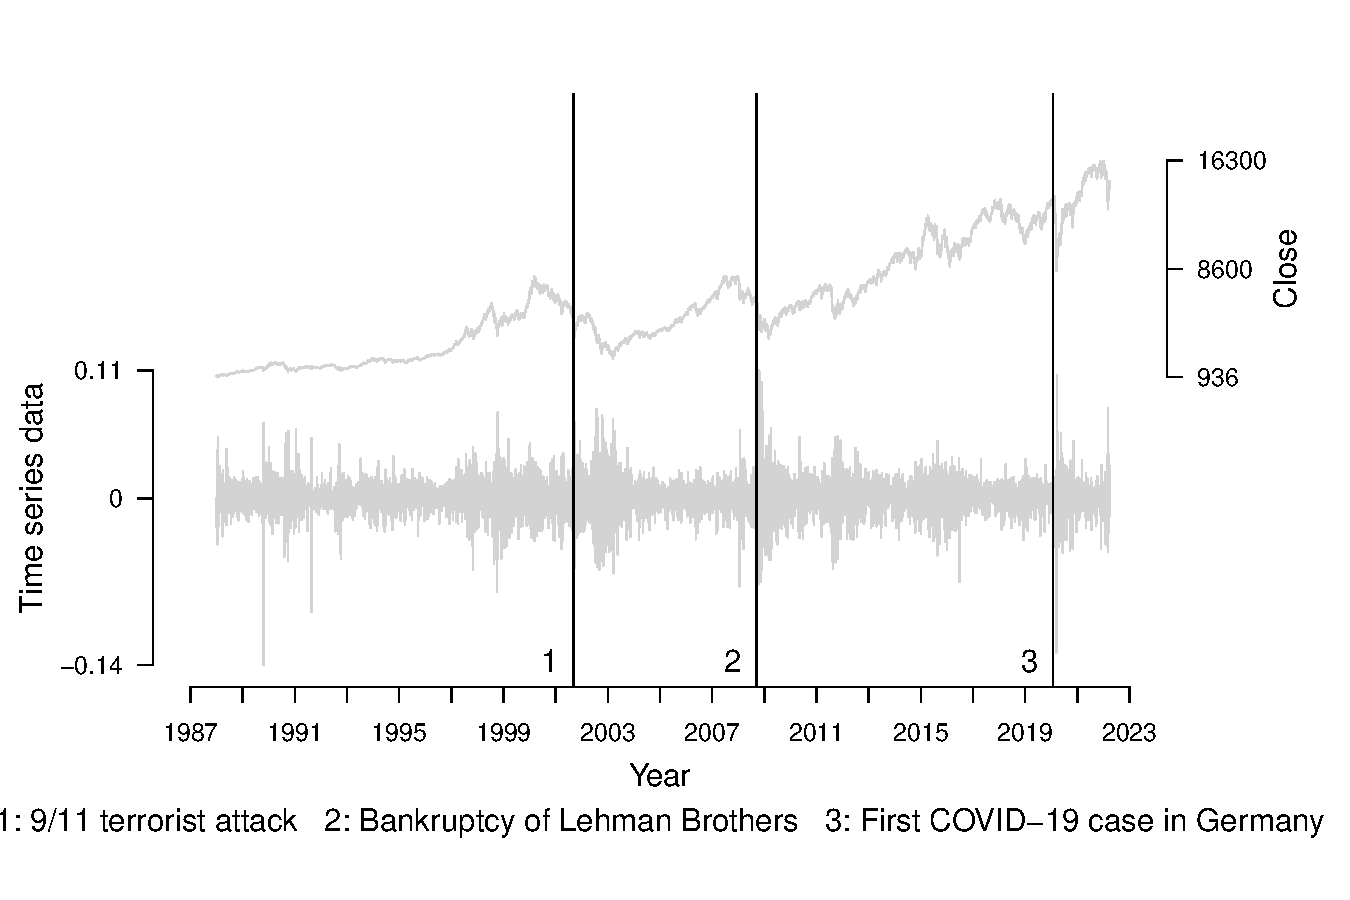
\includegraphics{fhmm_oelschlaeger_adam_michels-dax-ts}
%

\paragraph{Example 2: Simulation (cont.)}

As mentioned in the previous section, if the \code{data} parameter in the model's controls is unspecified, data is simulated from the model specification. True model parameters can be specified by defining an \class{fHMM\_parameters}-object via the \fct{fHMM\_parameters} function and passing it to \fct{prepare\_data}, for example:

%
\begin{Schunk}
\begin{Sinput}
R> pars <- fHMM_parameters(
+    controls = contr_sim, 
+    Gamma = matrix(c(0.9,0.2,0.1,0.8), nrow = 2), 
+    sigmas = c(0.1,0.5)
+  )
R> data_sim <- prepare_data(contr_sim, true_parameters = pars, seed = 1)
\end{Sinput}
\end{Schunk}
%

The visualization of the simulated time series shows the state persistence (induced by $\Gamma_{11} = 0.9$ and $\Gamma_{22} = 0.8$) and the different standard deviations ($\sigma_1 = 0.1$ and $\sigma = 0.5$) of the state-dependent Gamma distributions. Remember that the expectation values were fixed to $\mu_1 = 1$ and $\mu_2 = 2$.

%
\begin{Schunk}
\begin{Sinput}
R> plot(data_sim)
\end{Sinput}
\end{Schunk}
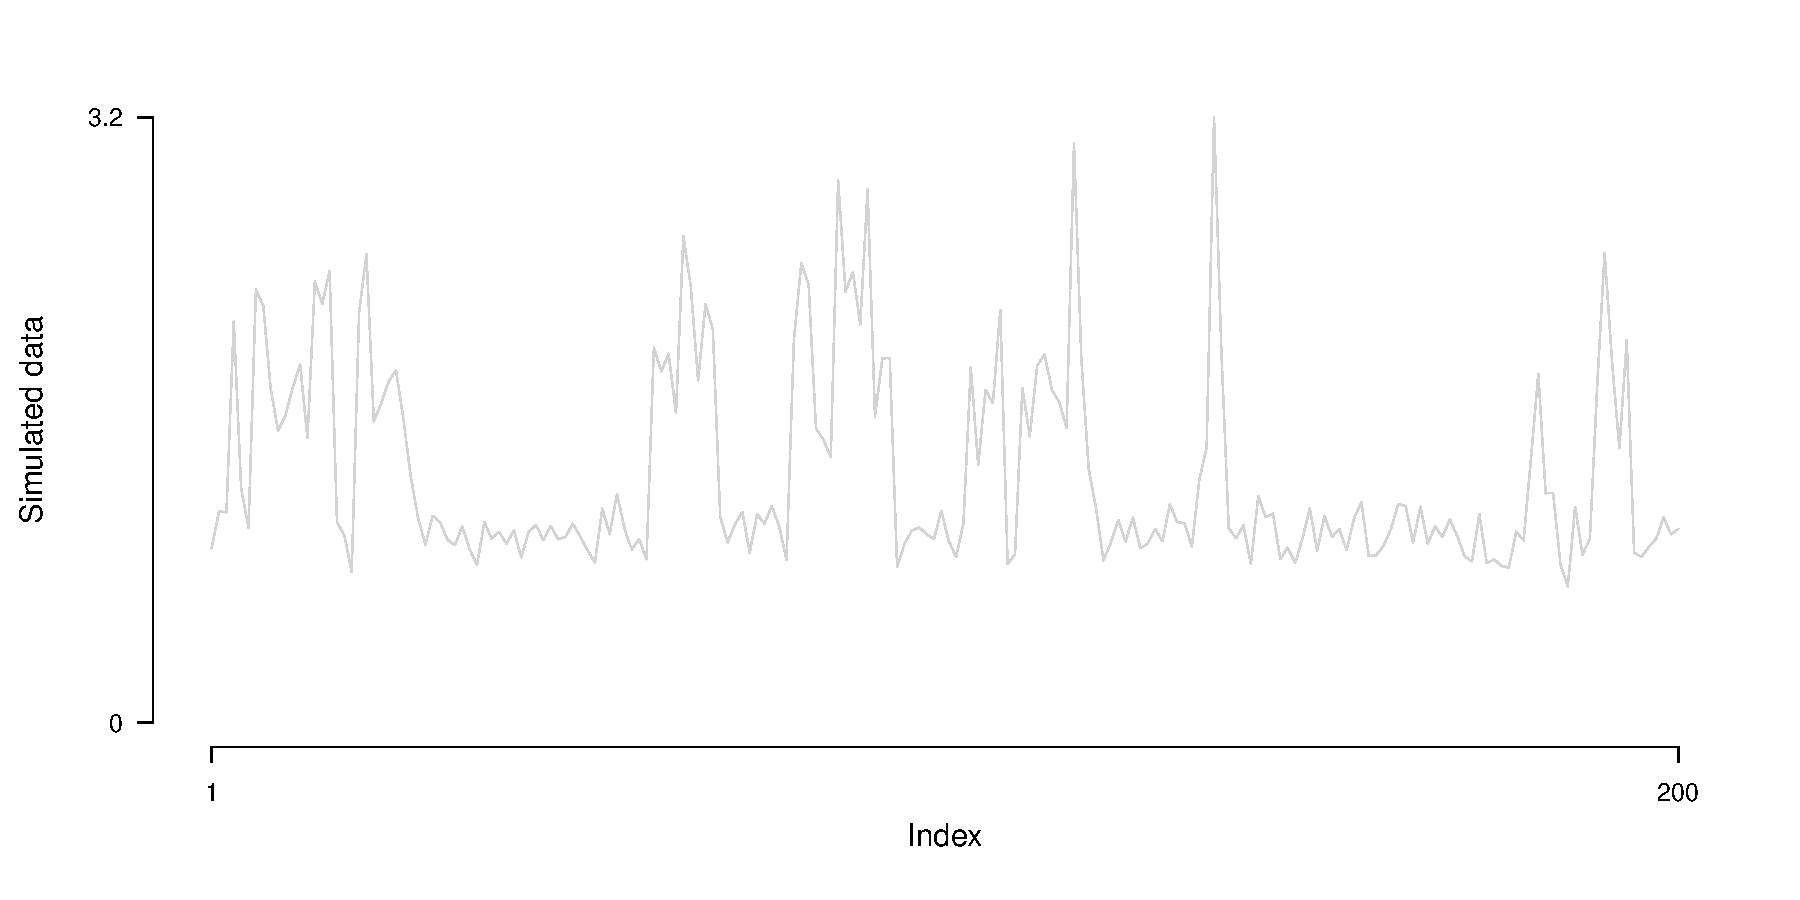
\includegraphics{fhmm_oelschlaeger_adam_michels-sim-data-ts}
%

\paragraph{Example 3: Hierarchy (cont.)}

Data preparation for the hiearchical case is analogue:

%
\begin{Schunk}
\begin{Sinput}
R> data_hhmm <- prepare_data(contr_hhmm)
\end{Sinput}
\end{Schunk}
%

\section{Model estimation} \label{sec:model_estimation} %% Timo + Lennart

The \pkg{fHMM} package applies the maximum-likelihood method for model estimation. The following derives the likelihood function of an HHMM, the non-hierarchical case can be deduced. We also discuss challenges in the numerical maximization and subsequently estimate the three running example models.

An HHMM can be treated as an HMM with two conditionally independent data streams; the coarse-scale observations on the one hand and the corresponding chunk of fine-scale observations connected to a fine-scale HMM on the other hand. To derive the likelihood of an HHMM, we start by computing the likelihood of each chunk of fine-scale observations being generated by each fine-scale HMM. 

To fit the $i$-th fine-scale HMM, with model parameters $\theta^{*(i)}=(\delta^{*(i)}, \Gamma^{*(i)},(f^{*(i,k)})_k)$ to the $t$-th chunk of fine-scale observations, which is denoted by $(X_{t,t^*})_{t^*}$, we consider the fine-scale forward probabilities 
\begin{align*}
\alpha^{*(i)}_{k,t^*}=f^{*(i)}(X^*_{t,1},\dots,X^*_{t,t^*}, S^*_{t,t^*}=k),
\end{align*}
where $t^*=1,\dots,T^*$ and $k=1,\dots,N^*$. Using the fine-scale forward probabilities, the fine-scale likelihoods can be obtained from the law of total probability as
\begin{align*}
\mathcal{L}^\text{HMM}(\theta^{*(i)}\mid (X^*_{t,t^*})_{t^*})=\sum_{k=1}^{N^*}\alpha^{*(i)}_{k,T^*}.
\end{align*}
The forward probabilities can be calculated recursively as
\begin{align*}
\alpha^{*(i)}_{k,1} &= \delta^{*(i)}_k f^{*(i,k)}(X^*_{t,1}), \\
\alpha^{*(i)}_{k,t^*} &= f^{*(i,k)}(X^*_{t,t^*})\sum_{j=1}^{N^*}\gamma^{*(i)}_{jk}\alpha^{*(i)}_{j,t^*-1}, \quad t^*=2,\dots,T^*.
\end{align*}

The transition from the likelihood function of an HMM to the likelihood function of an HHMM is straightforward: Consider the coarse-scale forward probabilities
\begin{align*}
\alpha_{i,t}=f(X_1,\dots,X_t,(X^*_{1,t^*})_{t^*},\dots,(X^*_{t,t^*})_{t^*}, S_t=i),
\end{align*}
where $t=1,\dots,T$ and $i=1,\dots,N$. The likelihood function of the HHMM results as
\begin{align*}
\mathcal{L}^\text{HHMM}(\theta,(\theta^{*(i)})_i\mid (X_t)_t,((X^*_{t,t^*})_{t^*})_t)=\sum_{i=1}^{N}\alpha_{i,T}.
\end{align*}
The coarse-scale forward probabilities can be calculated similarly:
\begin{align*}
\alpha_{i,1} &= \delta_i \mathcal{L}^\text{HMM}(\theta^{*(i)}\mid (X^*_{1,t^*})_{t^*})f^{(i)}(X_1), \\
\alpha_{i,t} &= \mathcal{L}^\text{HMM}(\theta^{*(i)}\mid (X^*_{t,t^*})_{t^*}) f^{(i)}(X_t)\sum_{j=1}^{N}\gamma_{ji}\alpha_{j,t-1}, \quad t=2,\dots,T.
\end{align*}

To account for parameter constraints associated with the transition probabilities (and potentially the parameters of the state-dependent distributions), we use parameter transformations. To ensure that the entries of the t.p.m.s fulfill non-negativity and the unity condition, we estimate unconstrained values $(\eta_{ij})_{i\neq j}$ for the non-diagonal entries of $\Gamma$ and derive the probabilities using the multinomial logit link
\begin{align*}
\gamma_{ij}=\frac{\exp(\eta_{ij})}{1+\sum_{k\neq i}\exp(\eta_{ik})},~i\neq j
\end{align*}
rather than estimating the probabilities $(\gamma_{ij})_{i,j}$ directly. The diagonal entries result from the unity condition as
\begin{align*}
\gamma_{ii}=1-\sum_{j\neq i}\gamma_{ij}.
\end{align*}
Furthermore, variances are strictly positive, which can be achieved by applying an exponential transformation to the unconstrained estimator.

Two more technical difficulties arise: First, we often face numerical under- or overflow, which can be addressed by maximizing the logarithm of the likelihood and incorporating constants in a conducive way, see \cite{oel21} for the details. Second, as the likelihood is maximized with respect to a relatively large number of parameters, the obtained maximum can be a local rather than the global one. To avoid this problem, it is recommended to run the maximization multiple times from different, possibly randomly selected starting points, and to choose the model that corresponds to the highest likelihood \citep{zuc16}. For efficient initialization, \pkg{fHMM} uses the first and second data moments as a basis for the initial guesses.

\paragraph{Example 1: DAX (cont.)} In section \ref{sec:data_management}, we defined the \class{fHMM\_data} object \code{data\_dax}. This object can be directly passed to the \fct{fit\_model} function that numerically maximizes the model's (log-) likelihood function:\footnote{The numerical maximization runs can be parallelized by setting the function's \code{ncluster} argument to a number greater than 1.}

%
\begin{Schunk}
\begin{Sinput}
R> dax_model_3t <- fit_model(data_dax)
\end{Sinput}
\end{Schunk}
%

The estimated model is saved in the \pkg{fHMM} package and can be accessed via:

%
\begin{Schunk}
\begin{Sinput}
R> data(dax_model_3t, package = "fHMM")
\end{Sinput}
\end{Schunk}
%

The \fct{coef} method returns a data frame of the estimated model coefficients along with 1-\code{alpha} confidence intervals (\code{alpha = 0.05} being the default) obtained via the inverse Fisher information (\code{lb} stands for lower- and \code{ub} upper-bound of the intervals, respectively):

%
\begin{Schunk}
\begin{Sinput}
R> coef(dax_model_3t, alpha = 0.05)
\end{Sinput}
\begin{Soutput}
                     lb      estimate           ub
Gamma_2.1  1.393745e-02  2.170056e-02 3.357222e-02
Gamma_3.1  1.710420e-06  1.696596e-06 1.671225e-06
Gamma_1.2  1.659146e-02  2.641008e-02 4.179228e-02
Gamma_3.2  9.359401e-03  1.740175e-02 3.213059e-02
Gamma_1.3  1.258535e-08  1.246159e-08 1.226657e-08
Gamma_2.3  2.789877e-03  5.145960e-03 9.431251e-03
mu_1       9.610235e-04  1.268712e-03 1.576400e-03
mu_2      -7.955275e-04 -2.517499e-04 2.920278e-04
mu_3      -3.723796e-03 -1.673649e-03 3.764982e-04
sigma_1    5.332119e-03  5.774343e-03 6.253244e-03
sigma_2    1.269075e-02  1.323801e-02 1.380887e-02
sigma_3    2.329677e-02  2.562622e-02 2.818860e-02
df_1       3.964154e+00  5.272157e+00 7.011747e+00
df_2       7.592272e+04  7.592547e+04 7.592821e+04
df_3       5.501298e+00  1.064107e+01 2.058285e+01
\end{Soutput}
\end{Schunk}
%

Adding \code{plot\_type = "sdds"} to the \fct{plot} method visualizes the estimated state-dependent distributions:

%
\begin{Schunk}
\begin{Sinput}
R> plot(dax_model_3t, plot_type = "sdds")
\end{Sinput}
\end{Schunk}
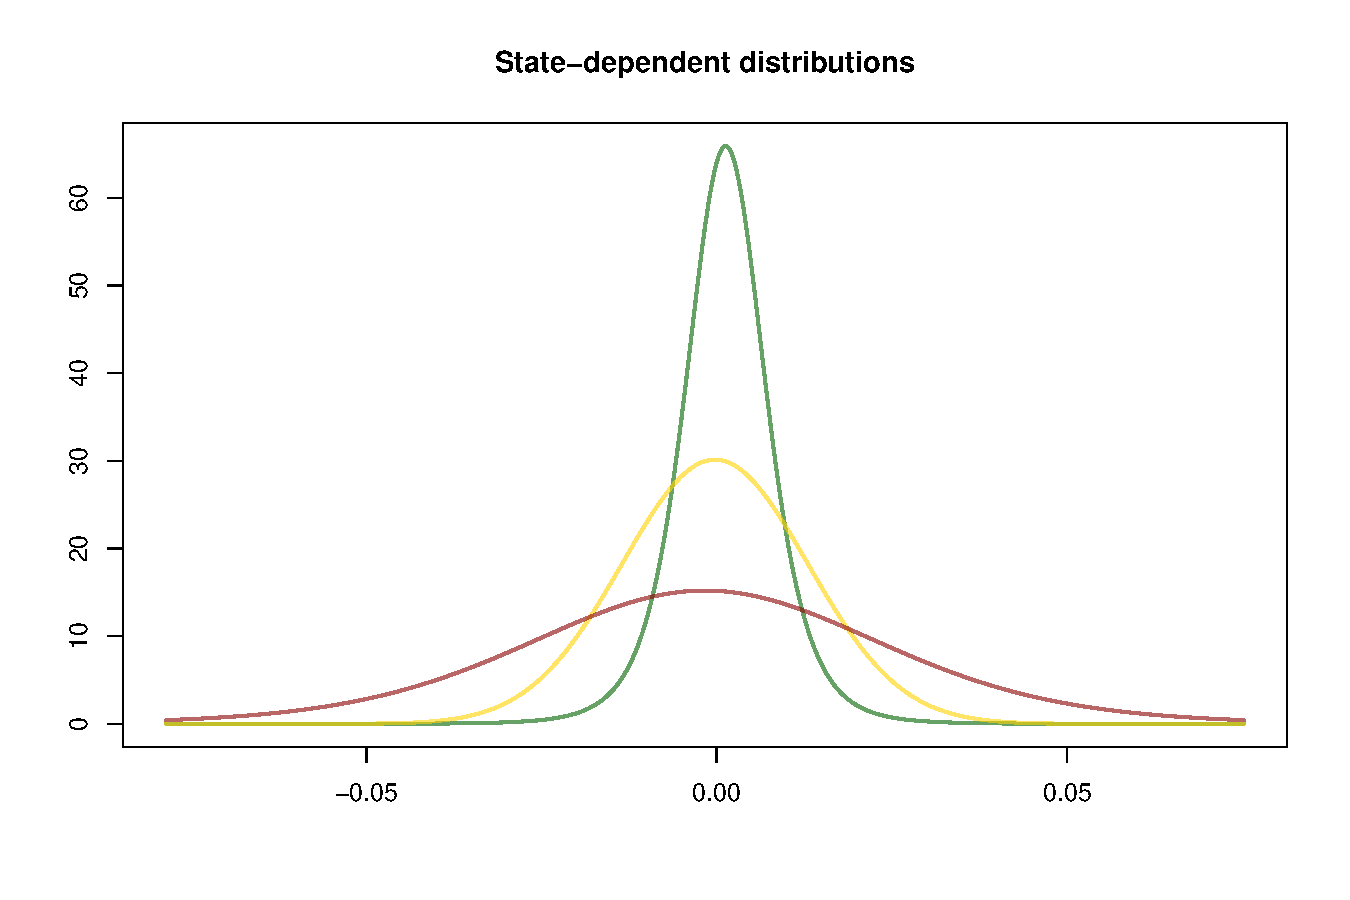
\includegraphics{fhmm_oelschlaeger_adam_michels-dax-sdds}
%

As mentioned above, the HMM likelihood function is prone to local optima. This effect can be visualized by plotting the log-likelihood values in the different optimization runs, where the best run is marked in red:

%
\begin{Schunk}
\begin{Sinput}
R> plot(dax_model_3t, plot_type = "ll")
\end{Sinput}
\end{Schunk}
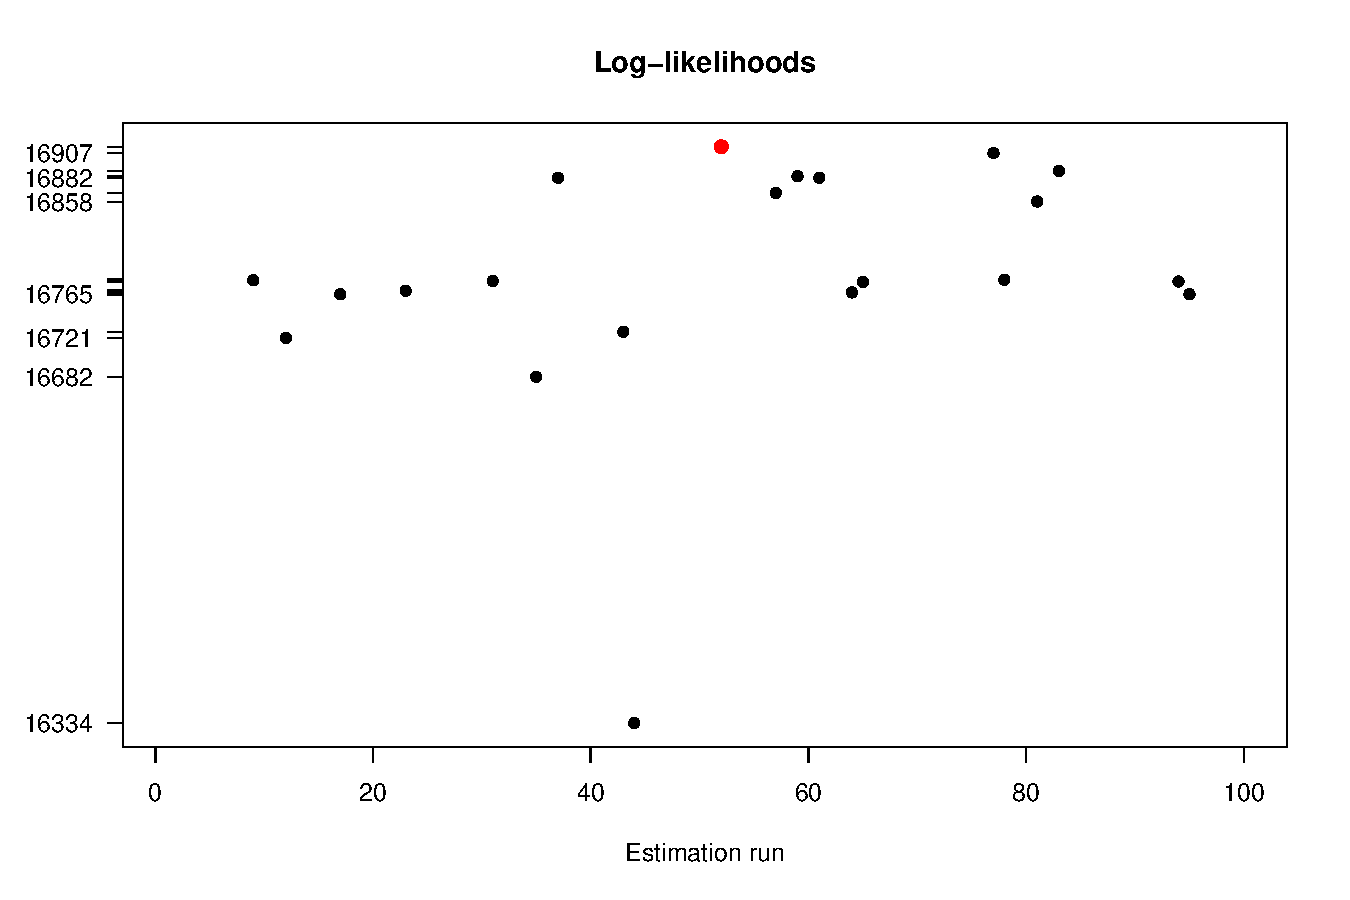
\includegraphics{fhmm_oelschlaeger_adam_michels-dax-ll}
%

\paragraph{Example 2: Simulation (cont.)} Fitting an HMM to the simulated data is analogue via the \fct{fit\_model} function. The estimated model \code{sim\_model\_2gamma} is also saved in \pkg{fHMM}: 

%
\begin{Schunk}
\begin{Sinput}
R> data(sim_model_2gamma, package = "fHMM")
\end{Sinput}
\end{Schunk}
%

The \fct{summary} method gives an overview of the estimated model. In the simulated case, we can compare the estimates to the true model coefficients:

%
\begin{Schunk}
\begin{Sinput}
R> summary(sim_model_2gamma)
\end{Sinput}
\begin{Soutput}
Summary of fHMM model

  simulated hierarchy        LL      AIC      BIC
1      TRUE     FALSE -192.9676 393.9353 407.1286

State-dependent distributions:
gamma(mu = 1|2) 

Estimates:
               lb estimate     ub true
Gamma_2.1 0.06475  0.17804 0.4039  0.2
Gamma_1.2 0.03052  0.07781 0.1844  0.1
sigma_1   0.44079  0.49962 0.5663  0.5
sigma_2   0.70108  0.92279 1.2146  1.0
\end{Soutput}
\end{Schunk}
%

\paragraph{Example 3: Hierarchy (cont.)}

In the hierarchical case, we can visualize the estimated state-dependent distributions on both the coarse-scale and the fine-scale layer:

%
\begin{Schunk}
\begin{Sinput}
R> # dax_vw_model <- fit_model(data_hhmm)
R> data(dax_vw_model, package = "fHMM")
R> plot(dax_vw_model, plot_type = "sdds")
\end{Sinput}
\end{Schunk}
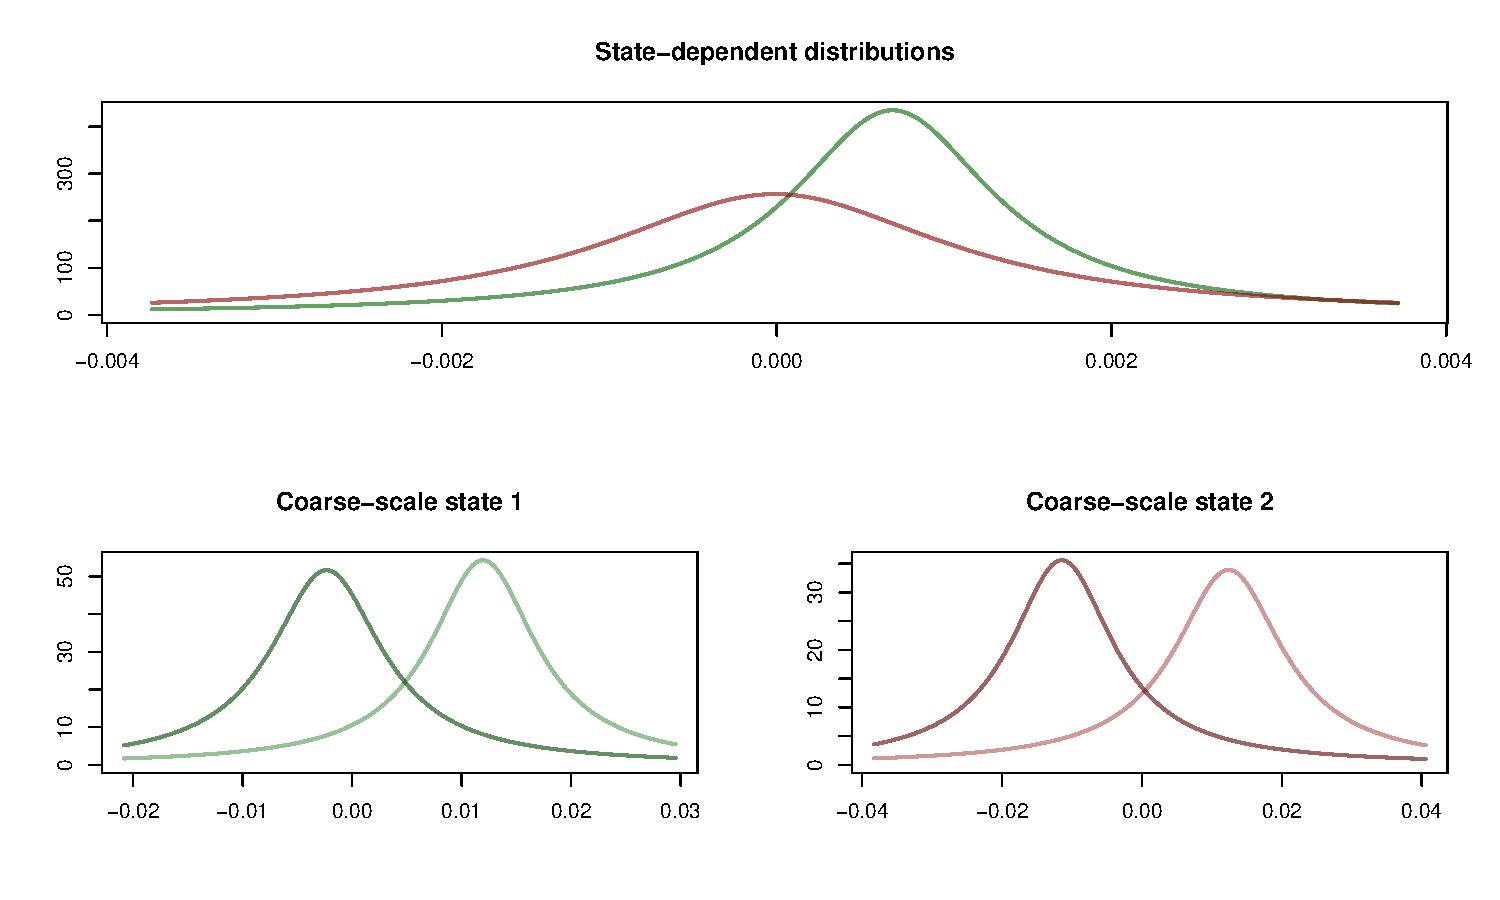
\includegraphics{fhmm_oelschlaeger_adam_michels-hhmm-sdds}
%

\section{State decoding and prediciton} \label{sec:state_decoding_and_prediction} %% Rouven + Lennart

For financial markets, it is of special interest to infer the underlying (hidden) states in order to gain insight about the actual market situation and for prediction. The Viterbi algorithm \citep{for73} is a recursive scheme that enables to find the most likely trajectory of hidden states under the estimated HMM. To this end, we follow \cite{zuc16} and define
\begin{align*}
  \zeta_{1i} &= \Pr(S_1 = i, X_1 = x_1) = \delta_i p_i(x_1) \\
  \zeta_{ti} &= \operatorname*{max}_{s_1, \ldots, s_{t-1}} \Pr(S_{t-1} = s_{t-1}, S_t = i, X_t = x_t)
\end{align*}
for $i = 1, \ldots, N$ (the index for the states) and $t = 2, \ldots, T$ (the index of time). Then, the trajectory of most likely states $i_1, \ldots, i_T$ can be calculated recursively backwards from
\begin{align*}
  i_T &= \operatorname*{argmax}_{i = 1, \ldots, N} \zeta_{Ti} \\
  i_t &= \operatorname*{argmax}_{i = 1, \ldots, N} (\zeta_{ti} \gamma_{i, i_{t+1}}), \quad t = T-1, \ldots, 1.
\end{align*}

Transferring the state decoding to HHMMs is straightforward via decoding the coarse-scale states first and afterwards, by using this information, decoding the fine-scale state process, see \cite{ada19}.

In the following, we introduce the \fct{decode\_states} function for state decoding and the \fct{predict} method for forecasting. As all of the \pkg{fHMM} functionalities presented in the remainder of this article are completely analogue for the hierarchical and the simulated case, respectively, we will focus our attention on example 1 and invite the reader to apply the methods to example 2 and 3 on their own. 

\paragraph{Example 1: DAX (cont.)} The underlying states of the 3-state HMM for the DAX can be decoded via the \fct{decode\_states} function, which updates an \class{fHMM\_model} object. 

%
\begin{Schunk}
\begin{Sinput}
R> dax_model_3t <- decode_states(dax_model_3t)
\end{Sinput}
\end{Schunk}
%

The state sequence is saved as argument \code{dax_model_3t$decoding}:

%
\begin{Schunk}
\begin{Sinput}
R> table(dax_model_3t$decoding)
\end{Sinput}
\begin{Soutput}
   1    2    3 
2177 2753  695 
\end{Soutput}
\end{Schunk}
%

The decoded time series can then be visualized via the \fct{plot} method:\footnote{Mind that the model is invariant to permutations of the state labels. \pkg{fHMM} provides the option to switch labels after decoding via the \fct{reorder\_states} function. For example \code{reorder\_states(dax\_model\_3t, 3:1)} reverses the order.}

%
\begin{Schunk}
\begin{Sinput}
R> plot(dax_model_3t)
\end{Sinput}
\end{Schunk}
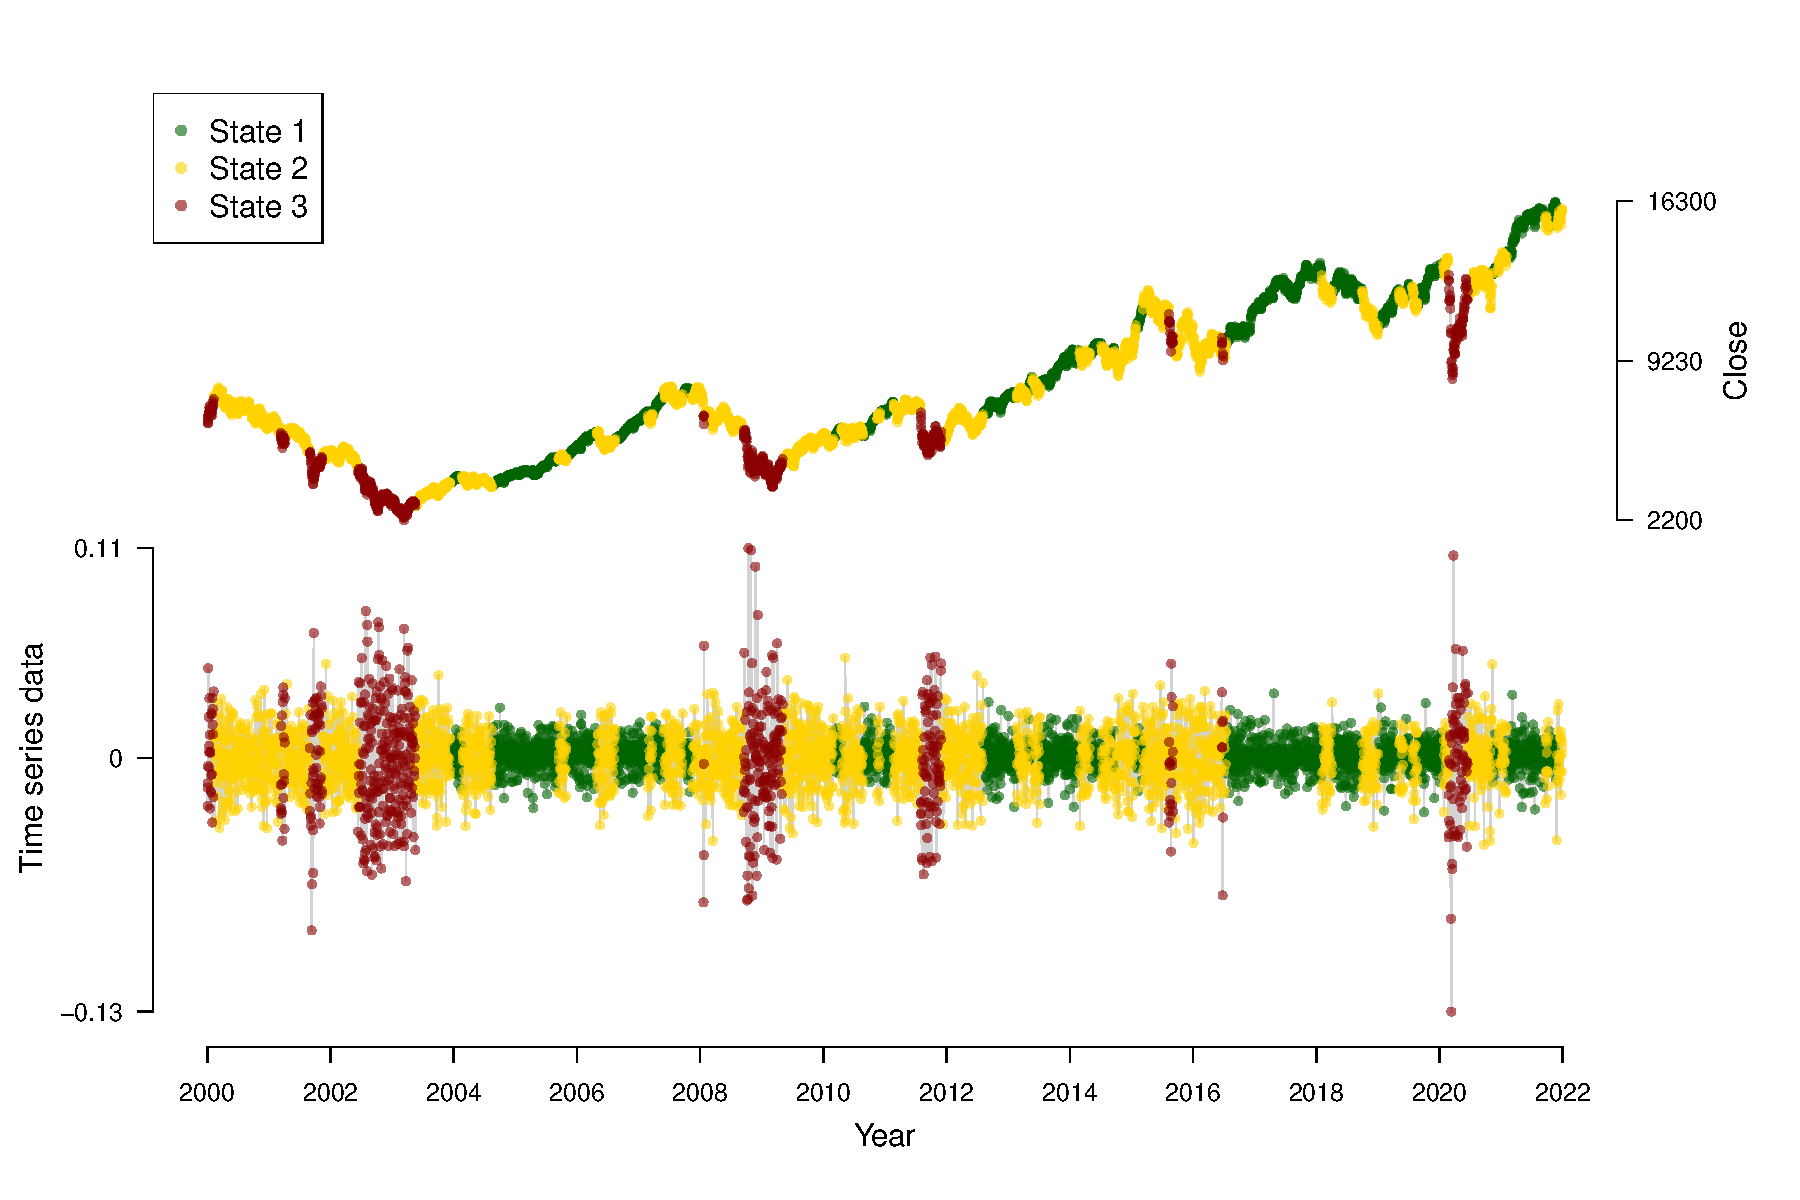
\includegraphics{fhmm_oelschlaeger_adam_michels-dax-dec-ts}
%

Having decoded the underlying states, we use the estimated transition probabilities to compute the state probabilities of next observations. Based on these probabilities and in combination with the estimated state-dependent distributions, upcoming observations can be predicted, compare \cite{zuc16}:

%
\begin{Schunk}
\begin{Sinput}
R> predict(dax_model_3t, ahead = 10)
\end{Sinput}
\begin{Soutput}
   state_1 state_2 state_3       lb estimate      ub
1  0.02170 0.97315 0.00515 -0.02190 -0.00023 0.02145
2  0.04225 0.94769 0.01006 -0.02179 -0.00020 0.02138
3  0.06170 0.92354 0.01477 -0.02168 -0.00018 0.02132
4  0.08011 0.90063 0.01926 -0.02158 -0.00016 0.02126
5  0.09754 0.87890 0.02356 -0.02148 -0.00014 0.02121
6  0.11403 0.85829 0.02767 -0.02140 -0.00012 0.02116
7  0.12965 0.83874 0.03161 -0.02131 -0.00010 0.02111
8  0.14442 0.82020 0.03537 -0.02124 -0.00008 0.02107
9  0.15841 0.80261 0.03898 -0.02116 -0.00007 0.02103
10 0.17164 0.78593 0.04243 -0.02110 -0.00005 0.02100
\end{Soutput}
\end{Schunk}
%

Columns 1 to 3 contain state probabilities for the next \code{ahead = 10} trading days. The values in columns 4 to 6 (the bounds of the 95\%-confidence intervals and the point predictions) are log-returns, which obviously can be transformed to index values or relative returns.

\section{Model checking} \label{sec:model_checking} %% Timo + Lennart

Checking whether a fitted model describes the data well is an essential part of any modeling process. In the HMM setting, this is typically done by analyzing so-called pseudo-residuals \citep{zuc16}. Since the observations are explained by different distributions (depending on the active state), they have to be transformed on a common scale as follows: If observation $X_t$ has the invertible distribution function $F_{X_t}$, then $Z_t=\Phi^{-1}(F_{X_t} (X_t))$ is standard normally distributed, where $\Phi$ denotes the cumulative distribution function of the standard normal distribution. The observations are modeled well if the pseudo-residuals $(Z_t)_t$ are approximately standard normally distributed and exhibit no autocorrelation. In the hierarchical case, we would first decode the coarse-scale state process using the Viterbi algorithm. Subsequently, we assign each coarse-scale observation its distribution function under the fitted model and perform the transformation described above. Using the Viterbi-decoded coarse-scale states, we then treat the fine-scale observations analogously.

\paragraph{Example 1: DAX (cont.)}

Via the \fct{compute\_residuals} function, pseudo-residuals can be computed in \pkg{fHMM} (provided that the states have been decoded beforehand). The function updates the \code{dax_model_3t} object in the following line:

%
\begin{Schunk}
\begin{Sinput}
R> dax_model_3t <- compute_residuals(dax_model_3t)
\end{Sinput}
\end{Schunk}
%

The normality and independence of the pseudo-residuals can be verified visually:

%
\begin{Schunk}
\begin{Sinput}
R> plot(dax_model_3t, plot_type = "pr")
\end{Sinput}
\end{Schunk}
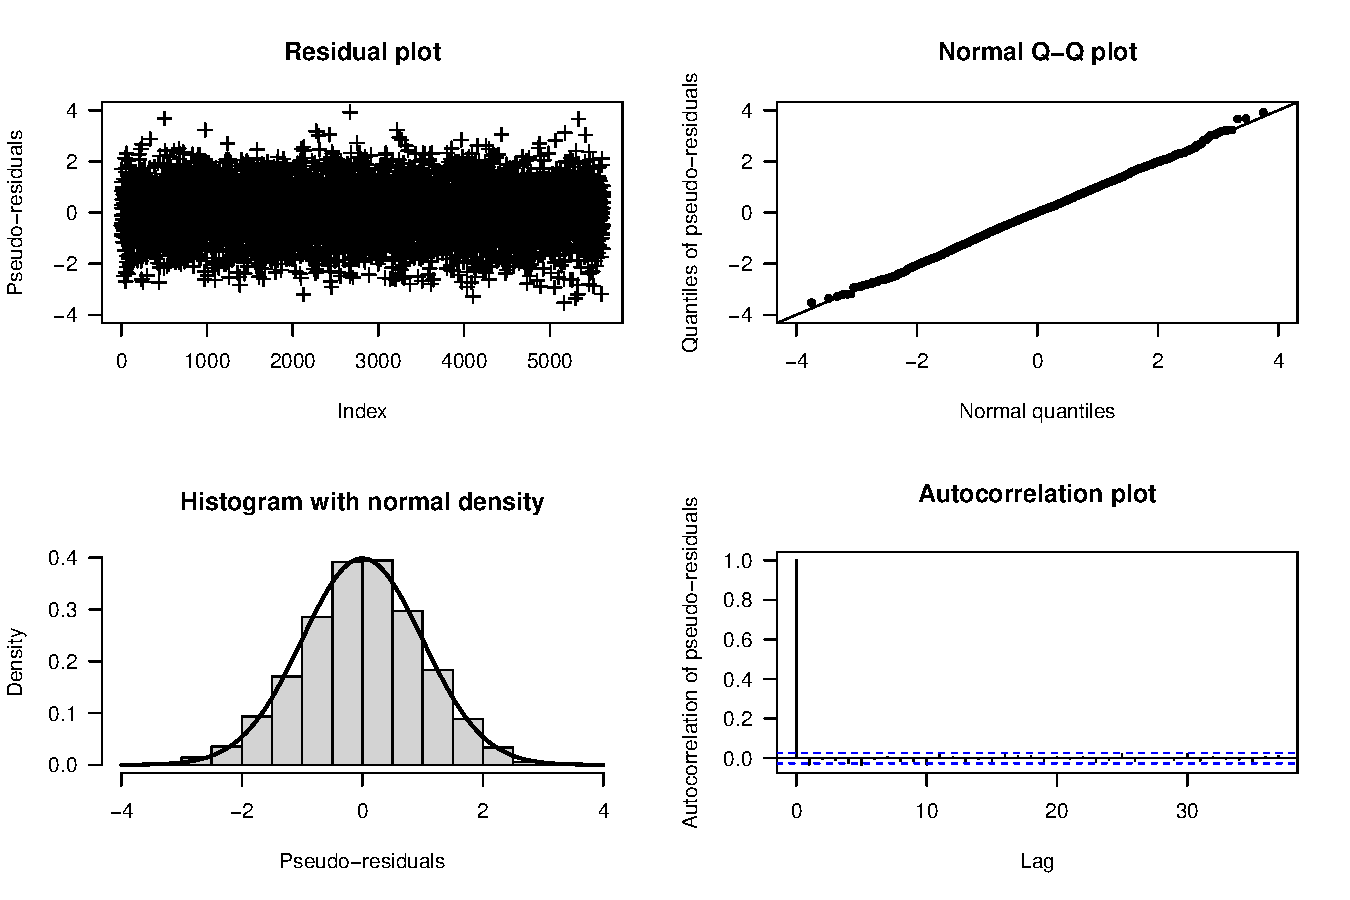
\includegraphics{fhmm_oelschlaeger_adam_michels-dax-res}
%

Alternatively, the residuals can be extracted from the model object for normality tests, for example a Jarque-Bera test \citep{jar87}:\footnote{Here, the test is unable to reject its null hypothesis that the data is normally distributed.}

%
\begin{Schunk}
\begin{Sinput}
R> res <- dax_model_3t$residuals
R> tseries::jarque.bera.test(res)
\end{Sinput}
\begin{Soutput}
	Jarque Bera Test

data:  res
X-squared = 2.6542, df = 2, p-value = 0.2652
\end{Soutput}
\end{Schunk}
%

\section{Model selection} \label{sec:model_selection} %% Timo + Lennart

Model selection involves the choice of a family for the state-dependent distributions and the selection of the number of states. Common model selection tools are information criteria, such as the Akaike information criterion (AIC) \citep{aka74} or the Bayesian information criterion (BIC) \citep{sch78}. They are defined as
\begin{align*}
\text{AIC} &= - 2 \log \mathcal{L}^\text{(H)HMM} + 2 p \\
\text{BIC} &= - 2 \log \mathcal{L}^\text{(H)HMM} + \log(T) p
\end{align*}
where $p$ denotes the number of parameters and $T$ the number of observations. Both criteria aim at finding a compromise between model fit and model complexity, where a model with a lower value is preferred. For an in-depth discussion of pitfalls, practical challenges, and pragmatic solutions regarding model selection, see \cite{poh17}. The \pkg{fHMM} package provides the \fct{compare\_models} function that takes (arbitrarily many) \class{fHMM\_model} objects as input and returns a matrix of the number of parameters, the log-likelihood value, the AIC, and the BIC. 

\paragraph{Example 1: DAX (cont.)} We compare our 3-state HMM DAX model with state-dependent t-distributions to an HMM with 2 states and normal state-dependent distributions. The competing model was estimated on the same data and can be accessed as object \code{dax_model_2n} from the package. AIC and BIC clearly prefer the more complex model:

%
\begin{Schunk}
\begin{Sinput}
R> data(dax_model_2n, package = "fHMM")
R> compare_models(dax_model_2n, dax_model_3t)
\end{Sinput}
\begin{Soutput}
             parameters log-likelihood       AIC       BIC
dax_model_2n          6       16681.98 -33351.96 -33312.15
dax_model_3t         15       16913.33 -33796.65 -33697.13
\end{Soutput}
\end{Schunk}
%

%% -- Summary/conclusions/discussion -------------------------------------------

\section{Conclusions} \label{sec:conclusion} % Timo + Rouven + Lennart

The \pkg{fHMM} package intends to make the estimation of hidden Markov models for financial time series data accessible to practitioners. It contains functionality for data download, model simulation, model fitting, state decoding, model checking, model selection, and visualization options. The package has a user-friendly design: model specification is centralized in a list of controls; four different package objects can be seamlessly passed between functions; the package usage follows a clear workflow (Figure \ref{fig:flowchart}). The paper presented this workflow on a basis of three examples (an application to index data, a model fitted to simulated data, and an hierarchical extension) that should enable the reader to tailor an HMM to their financial data.

Current package limitations include (1) the confined set of state-dependent distributions, (2) the restriction to a discrete state space and (3) to a discretized time dimension, (4) the limitation for a maximum number of two hierarchies, and (5) the need to specify the number of latent states in advance to the model estimation. We plan to overcome these limitation in future package versions.

%% -- Optional special unnumbered sections -------------------------------------

\section*{Computational details}

The results presented in this paper were obtained using
\proglang{R}~4.1.1 with the
\pkg{fHMM}~1.0.2 package. \proglang{R} itself
and all packages used are available from the Comprehensive
\proglang{R} Archive Network (CRAN) at \url{https://CRAN.R-project.org/}.


% \section*{Acknowledgments}

%% -- Bibliography -------------------------------------------------------------
%% - References need to be provided in a .bib BibTeX database.
%% - All references should be made with \cite, \citet, \citep, \citealp etc.
%%   (and never hard-coded). See the FAQ for details.
%% - JSS-specific markup (\proglang, \pkg, \code) should be used in the .bib.
%% - Titles in the .bib should be in title case.
%% - Journal titles should not be abbreviated and in title case.
%% - DOIs should be included where available.
%% - Software should be properly cited as well.

\bibliography{ref}


%% -- Appendix (if any) --------------------------------------------------------
%% - After the bibliography with page break.
%% - With proper section titles and _not_ just "Appendix".
% 
% \newpage
% 
% \begin{appendix}
% 
% \section{Installation} \label{app:installation}
% 
% \end{appendix}
% 
%% -----------------------------------------------------------------------------


\end{document}
